% Options for packages loaded elsewhere
\PassOptionsToPackage{unicode}{hyperref}
\PassOptionsToPackage{hyphens}{url}
%
\documentclass[
]{article}
\usepackage{lmodern}
\usepackage{amsmath}
\usepackage{ifxetex,ifluatex}
\ifnum 0\ifxetex 1\fi\ifluatex 1\fi=0 % if pdftex
  \usepackage[T1]{fontenc}
  \usepackage[utf8]{inputenc}
  \usepackage{textcomp} % provide euro and other symbols
  \usepackage{amssymb}
\else % if luatex or xetex
  \usepackage{unicode-math}
  \defaultfontfeatures{Scale=MatchLowercase}
  \defaultfontfeatures[\rmfamily]{Ligatures=TeX,Scale=1}
\fi
% Use upquote if available, for straight quotes in verbatim environments
\IfFileExists{upquote.sty}{\usepackage{upquote}}{}
\IfFileExists{microtype.sty}{% use microtype if available
  \usepackage[]{microtype}
  \UseMicrotypeSet[protrusion]{basicmath} % disable protrusion for tt fonts
}{}
\makeatletter
\@ifundefined{KOMAClassName}{% if non-KOMA class
  \IfFileExists{parskip.sty}{%
    \usepackage{parskip}
  }{% else
    \setlength{\parindent}{0pt}
    \setlength{\parskip}{6pt plus 2pt minus 1pt}}
}{% if KOMA class
  \KOMAoptions{parskip=half}}
\makeatother
\usepackage{xcolor}
\IfFileExists{xurl.sty}{\usepackage{xurl}}{} % add URL line breaks if available
\IfFileExists{bookmark.sty}{\usepackage{bookmark}}{\usepackage{hyperref}}
\hypersetup{
  pdftitle={STA360 Final Project},
  pdfauthor={Martin Lim; Michael Xue},
  hidelinks,
  pdfcreator={LaTeX via pandoc}}
\urlstyle{same} % disable monospaced font for URLs
\usepackage[margin=1in]{geometry}
\usepackage{graphicx}
\makeatletter
\def\maxwidth{\ifdim\Gin@nat@width>\linewidth\linewidth\else\Gin@nat@width\fi}
\def\maxheight{\ifdim\Gin@nat@height>\textheight\textheight\else\Gin@nat@height\fi}
\makeatother
% Scale images if necessary, so that they will not overflow the page
% margins by default, and it is still possible to overwrite the defaults
% using explicit options in \includegraphics[width, height, ...]{}
\setkeys{Gin}{width=\maxwidth,height=\maxheight,keepaspectratio}
% Set default figure placement to htbp
\makeatletter
\def\fps@figure{htbp}
\makeatother
\setlength{\emergencystretch}{3em} % prevent overfull lines
\providecommand{\tightlist}{%
  \setlength{\itemsep}{0pt}\setlength{\parskip}{0pt}}
\setcounter{secnumdepth}{-\maxdimen} % remove section numbering
\usepackage{booktabs}
\usepackage{longtable}
\usepackage{array}
\usepackage{multirow}
\usepackage{wrapfig}
\usepackage{float}
\usepackage{colortbl}
\usepackage{pdflscape}
\usepackage{tabu}
\usepackage{threeparttable}
\usepackage{threeparttablex}
\usepackage[normalem]{ulem}
\usepackage{makecell}
\usepackage{xcolor}
\ifluatex
  \usepackage{selnolig}  % disable illegal ligatures
\fi

\title{STA360 Final Project}
\author{Martin Lim \and Michael Xue}
\date{}

\begin{document}
\maketitle

\hypertarget{introduction}{%
\section{Introduction}\label{introduction}}

The Big Five personality trait model was developed by various individual
researchers. In 1936, Gordon Allport and Henry Odbert formed a list of
4,500 terms relating to personality traits, providing the foundation for
other psychologists to start investigating the basic dimensions of
personality. Using factor analysis, this list was eventually narrowed
down to five key personality traits, which became known as the ``Big
Five''. Each of these five traits actually encompasses a multitude of
other traits. For example, extraversion is an aggregate of
gregariousness, assertiveness, activity, excitement-seeking, positive
emotions, and warmth. Another key aspect of this Big Five model is that
it classifies personality traits on a spectrum, rather than into
specific categories. The Big Five traits are not associated with any
particular personality test, as there are several different ways to
measure these traits. Our project focuses on specifically on the
Big-Five Factor Markers from the International Personality Item Pool
developed by Lewis R. Goldberg. Overall, the Big Five personality trait
model can be useful for understanding the distribution of these traits
across particular populations of interest, and could thus inform policy
decisions, the general political climate, and more. In addition, this
analysis will give us insight into whether personality is a product of
both nature and nurture, or genetics and environment.

The goal of this project is to use Bayesian analysis to find a posterior
distribution that will capture close to the true distribution of scores
for the Big Five personality categories at the time of this study, using
a weakly informative prior and our dataset. In particular, we hope to
distribute our dataset into different classes based on continent in
order to see whether there are differences in these posterior
distributions potentially due to factors such as location and cultural
environment. While it may be hard to gain much insight on the aggregate,
we believe such analysis could be useful when focusing on specific
populations, such as how the personalities of teenagers in America are
changing over time (we can continually update our prior using Bayesian
analysis).

Our proposed Bayesian modeling framework will follow the MVN-MVN-IW
model as described in class. As such, we hope to use the data and a
weakly informative prior in order to generate a posterior that will
describe the mean vector for the score on each of the Big Five
personality traits and the corresponding covariance matrix. Our weakly
informative prior will essentially reflect our hypothesis that there are
no differences in personality across continents, and our posterior will
give us insight into whether these differences exist, and thus whether
environment can play a large role in determining overall trends of
personality.

\hypertarget{data}{%
\section{Data}\label{data}}

The data comes from the Open-Source Psychometrics Project, which
provides a collection of interactive personality tests. The data was
collected in 2012 through an online personality test of the Big-Five
Factor Markers from the International Personality Item Pool on the
Open-Source Psychometrics Project website. Prior to starting the test,
participants were informed that their responses would be recorded and
used for research purposes, and consent to record their responses was
confirmed after the test. This dataset contains 57 variables: 50 of
these variables are the participants' answers to the 50 question Big
Five personality test and 7 of these variables are additional
demographic information about the participant. The participants answer
the 50 questions on a scale of 1 to 5; 1 means that the participant
finds the statement ``Very Inaccurate'', 3 means that the statement is
``Neither Accurate Nor Inaccurate'', and 5 means that the statement is
``Very Accurate''; thus our data is ordinal discrete. The 7 demographic
variables that are not factored into the personality test are: race,
age, gender, handedness, the participant's country location, how the
participant came to the test, and whether English is the participant's
native language. The Big Five factors that this 50 question test
measures are (1) ``extraversion'', (2) ``agreeableness'', (3)
``conscientiousness'', (4) ``emotional stability'', and (5)
``intellect'' (for the purposes of modeling, we will observe this
ordering). Each question on the test corresponds to only one of these
factors, and each factor is defined by 10 questions.

The original dataset included 19719 observations, but 378 observations
were removed as they were missing the country variables. Given that each
observation is the result of just one participant, removing these
observations should not have any significant impact on our findings.
From the 50 questions, additional variables were created to store the
scores received in each of the Big Five factors. Scoring for the factors
is computed as follows: each question corresponds to a single factor and
is ``+keyed'' or ``-keyed''. For ``+keyed'' items, the response ``Very
Inaccurate'' is assigned a value of 1, ``Moderately Inaccurate'' a value
of 2, ``Neither Inaccurate nor Accurate'' a 3, ``Moderately Accurate'' a
4, and ``Very Accurate'' a value of 5. For ``-keyed'' items, the
response ``Very Inaccurate'' is assigned a value of 5, ``Moderately
Inaccurate'' a value of 4, ``Neither Inaccurate nor Accurate'' a 3,
``Moderately Accurate'' a 2, and ``Very Accurate'' a value of 1. Once
values are calculated for each question, they should be summed to obtain
the total score for that factor. Each factor can have a different number
of (``+keyed'', ``-keyed'') questions: extraversion (5, 5),
agreeableness (6, 4), conscientiousness (6, 4), emotional stability (2,
8), intellect (3, 7). After obtaining a score for each factor on each
observation, we found that scores were normally distributed for each
factor, with agreeableness and intellect being a little left skewed.

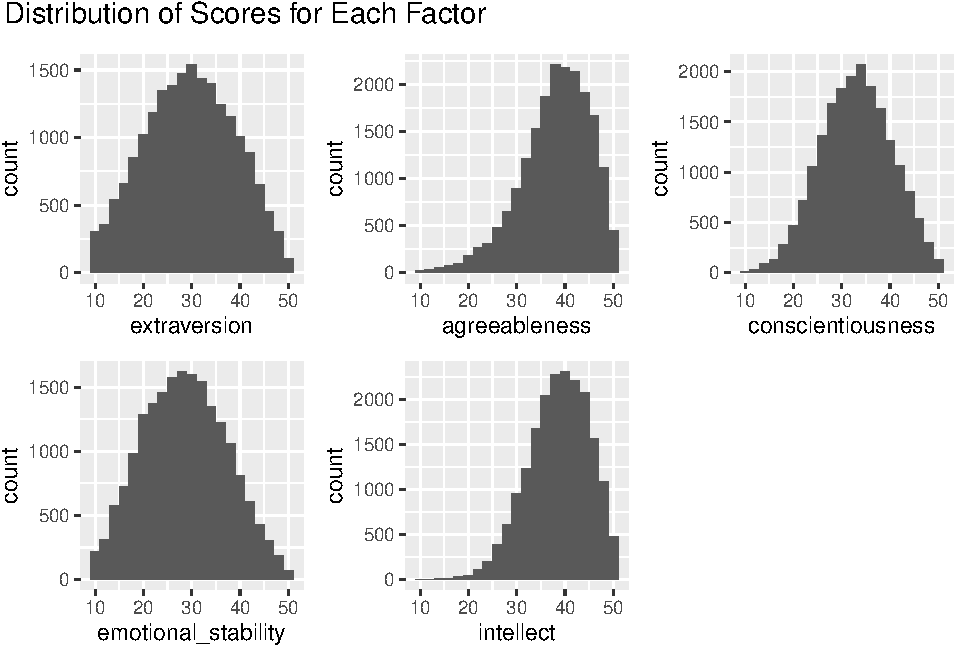
\includegraphics{project_files/figure-latex/unnamed-chunk-6-1.pdf}

A limitation of the data is that the country variable represents the
country in which the participant is taking the test from, which is not
necessarily their country of residence. However, we can assume that the
country variable does represent the country of residence of the
participant in the vast majority of cases. Another limitation of the
data is that these participants are most likely not going to be
representative of the total population in these countries or continents.
The participants represent those in these countries and continents who
have access to internet and a device and are inclined to take such a
personality test in English. A strength of our data from a modeling
perspective is that the distribution of scores for personality
categories is likely to be normally distributed.

In order to perform our Bayesian analysis on each of the continents
separately, we must group our data frame by continent by using the
country codes. To find the continent codes for each country, we imported
a data frame from an outside source mapping country code to the
corresponding continent code. We merged the two data frames together and
selected only the necessary variables. The continents represented in the
final data are North America (NA), Europe (EU), Asia (AS), Oceania (OC),
Africa (AF), and South America (SA).

\setlength{\tabcolsep}{6pt}
 \begin{table}
\centering

\label{tab:unnamed-chunk-7}\begin{tabular}{ll}
  \multicolumn{1}{l}{Continent} & \multicolumn{1}{l}{Count}   \\ 
 \multicolumn{1}{l}{NA} & \multicolumn{1}{l}{9899}   \\ 
 \multicolumn{1}{l}{EU} & \multicolumn{1}{l}{4039}   \\ 
 \multicolumn{1}{l}{AS} & \multicolumn{1}{l}{3623}   \\ 
 \multicolumn{1}{l}{OC} & \multicolumn{1}{l}{1140}   \\ 
 \multicolumn{1}{l}{AF} & \multicolumn{1}{l}{394}   \\ 
 \multicolumn{1}{l}{SA} & \multicolumn{1}{l}{292}   \\ 

 \end{tabular}
\end{table}

\hypertarget{modeling}{%
\section{Modeling}\label{modeling}}

Our proposed Bayesian model framework is the MVN-MVN-IW (Multivariate
Normal - Multivariate Normal - Inverse Wishart) model. This is because
we assume our covariance matrix to be unknown, and we see in the EDA
that the distribution of the score of each category seems to be roughly
normal. Thus, it would make sense to model the vector of scores as a
mean vector, and have the covariance matrix represent the variances of
the categories on the diagonal and the covariances of the categories on
the nondiagonals (it is possible for some of the categories to be
correlated with one another, such as intellect and conscientiousness).
In this framework, we have two independent priors,
\(\boldsymbol \theta \sim MVN(\boldsymbol \mu, \boldsymbol T)\) and
\(\mathbf\Sigma \sim IW(\Psi, \nu)\). Our sampling model will be a
Multivariate Normal, such that
\(y_i \sim MVN(\boldsymbol \theta, \mathbf\Sigma)\). As we want to
create a weakly informative prior, we will assume the following:

\begin{enumerate}
\def\labelenumi{\arabic{enumi}.}
\tightlist
\item
  Each continent \(i \in (1, 6)\) has the same mean for each of the Big
  Five personality trait scores. We will set this to be 30, since each
  category has 10 questions with a presumed average value of 3 (neutral
  response on a scale of 1-5). Thus, our prior value of
  \(\boldsymbol \mu = [30, 30, 30, 30, 30]\).
\item
  The Big Five personality traits are uncorrelated with one another.
  Thus we will set the off-diagonals of the prior for \(\mathbf T\) and
  \(\Psi\) to be 0. Note that we assume our priors for \(\mathbf T\) and
  \(\Psi\) to be the same.
\item
  Each category's variance for score will be equal. We calculate this
  via the following. Let \(Y\) be a random variable denoting the total
  score for one of the Big Five personality categories. Since each
  category's score is determined by ten questions, we can write
  \(Y = X_1 + ... + X_{10}\), where each \(X_i \sim U\{1,5\}\), where
  \(X_i\) represents the score obtained for the \(i\)'th question, and
  \(U\{a,b\}\) represents a Discrete Uniform distribution for values
  \(a, a+1, ..., b-1, b\). In other words, we assume each \(X_i\) is
  equally likely to be assigned scores between 1 and 5. Given that the
  variance of a Discrete Uniform is given by \(\frac{n^2 - 1}{12}\),
  where \(n = b - a + 1\), and we assume a weak positive correlation of
  \(Corr(X_i, X_j) = 0.7\) for all \(i \neq j\) (since each of these
  questions are within the same category, we can assume that scores for
  one question would be positively correlated with those for another),
  we derive the following: \[
  \begin{aligned}
  Var(Y) &= Var(X_1 + ... + X_{10})\\
  &= \sum_{i=1}^{10} Var(X_i) + \sum_{i \neq j} Cov(X_i, X_j)\\
  &= 10 * \frac{5^2-1}{12} + 90 * 0.7 * \frac{5^2-1}{12}\\
  &= 146
  \end{aligned}
  \]
\end{enumerate}

Thus, in our prior for \(\mathbf T\) and \(\Psi\), we will set the
diagonals to be 146.

\begin{enumerate}
\def\labelenumi{\arabic{enumi}.}
\setcounter{enumi}{3}
\tightlist
\item
  Our prior for \(\nu\) will be the minimum sample size that still
  satisfies \(\nu > d - 1\), so we set \(\nu = 5\).
\end{enumerate}

Now that we have established our priors, our modeling procedure is
straightforward. As we cannot find a closed form expression for the
posterior, we derive the full conditionals for \(\boldsymbol \theta\)
and \(\mathbf\Sigma\) and find the following expressions for them:

\[\boldsymbol{\theta} \sim MVN(\boldsymbol{\mu}^*(\mathbf{\Sigma}), \mathbf{T}^*(\mathbf{\Sigma})) \text{, where}\]
\[\boldsymbol{\mu}^*(\mathbf{\Sigma}) = (\mathbf{T}^{-1} + n \mathbf{\Sigma}^{-1})^{-1} (n \mathbf{\Sigma}^{-1} \bar{\mathbf{y}} + \mathbf{T}^{-1} \boldsymbol{\mu})\]
\[\mathbf{T}^*(\mathbf{\Sigma}) = (\mathbf{T}^{-1} + n\mathbf{\Sigma}^{-1})^{-1}\]
\[\text{and}\]
\[\mathbf{\Sigma} \sim IW(\Psi^* (\boldsymbol{\theta}), \nu^*) \text{, where}\]
\[\Psi^* (\boldsymbol{\theta}) = \Psi + n\mathbf{S}(\boldsymbol{\theta})\]
\[\mathbf{S}(\boldsymbol{\theta}) = \frac{1}{n} \sum_{i=1}^n (\mathbf{y}_i - \boldsymbol{\theta}) (\mathbf{y}_i - \boldsymbol{\theta})^T\]
\[\nu^* = \nu + n\] For each of the six continents we are investigating,
we can then run a Gibbs sampler to find our posterior samples of
\(\boldsymbol \theta\) and \(\mathbf \Sigma\). We note that the
autocorrelation and trace plots in the Appendix suggest that our Gibbs
sampler is quite effective at producing independent samples. We provide
an example autocorrelation and trace plot for the extraversion category
in North America in the results section.

We then perform a predictive check to compare this distribution of
scores with the distribution of scores reflected in the data. To do so,
we take the posterior samples of \(\boldsymbol \theta\) and
\(\mathbf \Sigma\), use our sampling model (MVN) with those parameters
to get predictive samples, and plot density plots for each category for
each continent. Our goal here is to check that our modeling approach is
sound by making sure that the predictive distributions do not deviate
too far from the data; in fact, they should be close to the
distributions of the data given our weakly informative prior.

In addition, we hope to use our predictive distributions to give us
insight into our initial research question of whether the scores for
these personality traits differ between continents. We can get an
initial idea of this through our density plots, as well as confidence
intervals for the scores of each trait for each continent. To look into
this further, however, we can use our predictive samples to calculate
probabilities that the scores of a certain trait differ between
continents. Based on our predictive density plots, as well as our
initial data density plots, some questions we seek to answer are:

\begin{enumerate}
\def\labelenumi{\arabic{enumi}.}
\tightlist
\item
  Do people in North America score higher on extraversion compared to
  people in South America?
\item
  Do people in Africa score higher on conscientiousness compared to
  people in South America?
\item
  Do people in South America score higher on intellect compared to
  people in Asia?
\end{enumerate}

\hypertarget{results}{%
\section{Results}\label{results}}

An example autocorrelation and trace plot for the extraversion category
in North America is shown below.

\includegraphics{project_files/figure-latex/unnamed-chunk-9-1.pdf}
\includegraphics{project_files/figure-latex/unnamed-chunk-10-1.pdf}

As we can see, our Gibbs sampler mixes quite well and has low
autocorrelation, so we can assume that our samples are relatively
independent of one another. Because our Gibbs sampler seems to converge
very quickly, we decided that a burn-in period would not be necessary.

Using the posterior distribution of \(\boldsymbol \theta\) and
\(\mathbf \Sigma\), we sampled from the multivariate normal distribution
to obtain the predictive distribution of scores in each personality
category for each continent. The density plots for these predictive
distributions are shown below.

\includegraphics{project_files/figure-latex/unnamed-chunk-11-1.pdf}

In comparison to the density plots for the distribution of data we
showed earlier, these predictive distributions roughly match in terms of
mean and range. Thus, our predictive check is passed. However, these
predictive distributions are more normal, whereas the data density plots
have some skewed behavior for agreeableness and intellect. This is a
limitation of the MVN-MVN-IW model, as it influences the posterior and
predictive distributions to reflect a more normal shape. Another
limitation is that for several of the continents, such as North America
and Europe, the large number of observations causes the data to take
significantly more precedence than the prior, and so our predictive
distribution will naturally be very close to the distribution of the
data itself. On the other hand, there is a discrepancy in the effect of
the prior on our model between continents, as continents such as Africa
and South America have much fewer observations.

Below are the various \(95\%\) confidence intervals for each of the
personality category scores for each continent.

\setlength{\tabcolsep}{6pt}
 \begin{table}
\centering

\label{tab:unnamed-chunk-12}\begin{tabular}{lllll}
  \multicolumn{1}{l}{extraversion} & \multicolumn{1}{l}{agreeableness} & \multicolumn{1}{l}{conscientiousness} & \multicolumn{1}{l}{em_stability} & \multicolumn{1}{l}{intellect}   \\ 
 \multicolumn{1}{l}{(11.49, 49.08)} & \multicolumn{1}{l}{(24.69, 53.15)} & \multicolumn{1}{l}{(19.35, 48.82)} & \multicolumn{1}{l}{(12.05, 46.91)} & \multicolumn{1}{l}{(27.26, 51.87)}   \\ 
 \multicolumn{1}{l}{(12.20, 48.59)} & \multicolumn{1}{l}{(23.01, 52.34)} & \multicolumn{1}{l}{(18.39, 46.12)} & \multicolumn{1}{l}{(11.35, 45.53)} & \multicolumn{1}{l}{(28.02, 51.74)}   \\ 
 \multicolumn{1}{l}{(13.55, 45.03)} & \multicolumn{1}{l}{(25.92, 49.51)} & \multicolumn{1}{l}{(19.92, 46.81)} & \multicolumn{1}{l}{(12.46, 43.23)} & \multicolumn{1}{l}{(24.86, 48.89)}   \\ 
 \multicolumn{1}{l}{(12.11, 49.38)} & \multicolumn{1}{l}{(24.45, 52.71)} & \multicolumn{1}{l}{(17.46, 46.94)} & \multicolumn{1}{l}{(12.55, 45.95)} & \multicolumn{1}{l}{(27.00, 51.58)}   \\ 
 \multicolumn{1}{l}{(12.84, 47.42)} & \multicolumn{1}{l}{(25.30, 53.32)} & \multicolumn{1}{l}{(20.70, 49.81)} & \multicolumn{1}{l}{(12.39, 48.17)} & \multicolumn{1}{l}{(27.35, 51.64)}   \\ 
 \multicolumn{1}{l}{(9.15, 44.13)} & \multicolumn{1}{l}{(21.01, 50.02)} & \multicolumn{1}{l}{(16.33, 43.77)} & \multicolumn{1}{l}{(11.90, 42.65)} & \multicolumn{1}{l}{(28.63, 52.65)}   \\ 

 \end{tabular}
\end{table}

From our initial observations of the predictive density plots as well as
the confidence intervals, there does not seem to be a significant
difference in the distributions of personality category scores between
continents. To confirm this, we will answer three of the questions we
posed above.

\begin{verbatim}
## [1] 0.6084
\end{verbatim}

\begin{verbatim}
## [1] 0.6848
\end{verbatim}

\begin{verbatim}
## [1] 0.661
\end{verbatim}

Let \(A\) represent the event that a predictive sample of extraversion
score in North America is greater than a predictive sample of
extraversion score in South America.

Let \(B\) represent the event that a predictive sample of
conscientiousness score in Africa is greater than a predictive sample of
conscientiousness score in South America.

Let \(C\) represent the event that a predictive sample of intellect
score in South America is greater than a predictive sample of intellect
score in Asia.

Calculating these probabilities, we find that: \[P(A) = 0.6084\]
\[P(B) = 0.6848\] \[P(C) = 0.661\] Based on the probability of these
events, there is some, but perhaps not significant, evidence that the
scores for these traits may differ between specific continents. This may
suggest that different environments in continents could be responsible
for these discrepancies. This could be useful to psychologists and
cultural anthropologists who are investigating how different
environments or other factors could affect the development of people's
personalities and specific traits.

\hypertarget{conclusion}{%
\section{Conclusion}\label{conclusion}}

Overall, our key findings are that prior research suggesting the impact
of genetics and the environment on the Big Five personality traits is
true to some extent, as we saw in our analysis. However, these
differences are not clearly significant across continents. Nonetheless,
our project may provide psychologists and cultural anthropologists with
some useful information for how to analyze the effect of a certain
variable on the development of people's personalities.

Our project specifically looked into these personality differences
across continents as our varying feature. However, other variables were
also provided, such as age, gender, and whether English is the person's
native language. A similar analysis as the one we have conducted in this
project can be extended to these features as well, and more
investigation should be done in order to determine what factors in
particular have the largest effects on the development (or lack thereof)
of the Big Five personality traits.

\hypertarget{appendix}{%
\section{Appendix}\label{appendix}}

\includegraphics{project_files/figure-latex/trace-1.pdf}
\includegraphics{project_files/figure-latex/trace-2.pdf}
\includegraphics{project_files/figure-latex/trace-3.pdf}
\includegraphics{project_files/figure-latex/trace-4.pdf}
\includegraphics{project_files/figure-latex/trace-5.pdf}
\includegraphics{project_files/figure-latex/trace-6.pdf}
\includegraphics{project_files/figure-latex/trace-7.pdf}
\includegraphics{project_files/figure-latex/trace-8.pdf}
\includegraphics{project_files/figure-latex/trace-9.pdf}
\includegraphics{project_files/figure-latex/trace-10.pdf}
\includegraphics{project_files/figure-latex/trace-11.pdf}
\includegraphics{project_files/figure-latex/trace-12.pdf}

\end{document}
